\chapter{Network architectures}
	\label{CH_03}


\section{Overall architecture}
Z.Li et al. \cite{Z.Li2016} proposed a deep convolutional and recurrent neural network for predicting protein secondary structure. In their work a multiscale convolutional layer is followed by bidirectional GRU recurrent layers. In this work, I follow their general architecture as illustrate in Figure \ref{fig:overall_arch} which have preprocessing, multiscale convolution, recurrent and output four major parts. More details of these parts are explained in the following sections.
\begin{figure}[H] 
	\centering
	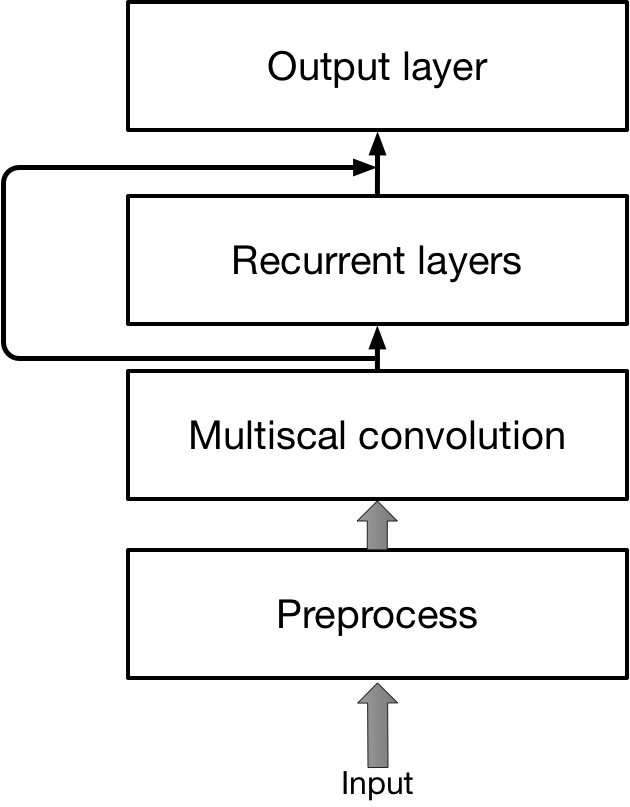
\includegraphics[width=3in]{Figures/overall_architecture}
	\caption[Detail inside recurrent unit]{Illustration of recurrent network}
	\label{fig:overall_arch}
\end{figure}

\section{Input and output}
\subsection{Input}
The input of the network have the shape of [sequence\_length, features]. In this work the number of features is 42, which contains two parts. For each amino acid in the sequence, the first 21 features is a one-hot-encoding indicate which amino acid it is. The last 21 features are the profiles features obtained from PSI-BLAST\cite{altschul1997gapped} which is a dense vector.
\subsection{Output}
The output the network have the shape of [sequence\_length, 8]. So for each amino acid in the sequence it will output a one-hot-encoding to indication which secondary structure it is.


\section{Preprocessing}
As illustrate in Figure \ref{fig:pre} What the preprocessing module does is converting the sparse one-hot-encoding of amino acid to a dense representation, and merge it with the dense profile feature vector. In order to avoid the inconsistency of feature representations. Same as the original work, a 21-by-50 embedding matrix is used. 
Another poteintial benefit of using a embedding matrix is we can initialize the embedding matrix with a pretrained matrix which comes from a sequence auto-encoder.

\begin{figure}[H] 
	\centering
	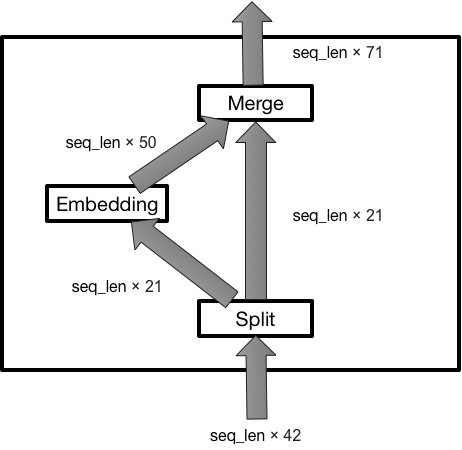
\includegraphics[width=3in]{Figures/preprocessing}
	\caption[Detail inside recurrent unit]{Illustration of recurrent network}
	\label{fig:pre}
\end{figure}

\section{Multiscale convolution}
After getting embedded features, the next step is using different 1-D convolutional kernels to extract loacl context information from the sequence. As shown in Figure \ref{fig:multi_conv}, total three kernels are used. Each of them have 64 output channels. And the shape of the kernel are 3, 7, 11 respectively. The kernel will moving along the protein with stride size 1. A concatenate layer will merge the output of three convolution layers and then a RELU layer will generate the activation. So far the module is the same as the one in original work. However in this work, a batch normalization layer is added after the activation. This layer will normalize the output of the module to have same distribution at each position and speed up the converging make the network learn faster. However, while learning faster, the model is more likely to overfit. Thus a dropout layer will also add at the end of this module.\par
\begin{figure}[H] 
	\centering
	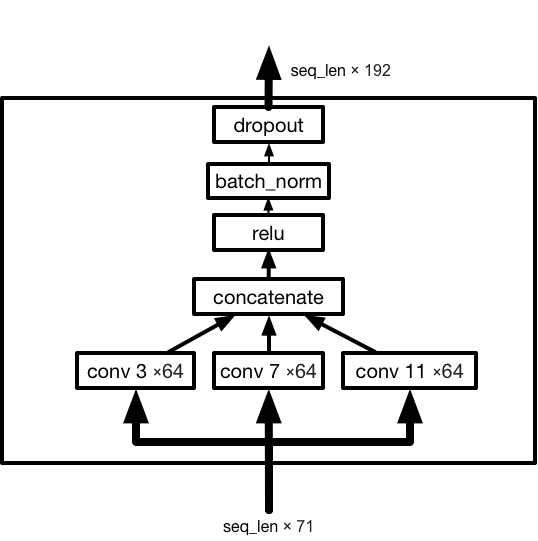
\includegraphics[width=3in]{Figures/multiscale_conv}
	\caption[Detail inside recurrent unit]{Illustration of recurrent network}
	\label{fig:multi_conv}
\end{figure}

\section{Recurrent layers}
In addition to the local dependency extracted by convolutional network, Z.Li et al. \cite{Z.Li2016} argued that long-range dependency is also important for secondary structure prediction. However a convolutional layer can not capture dependencies that longer than the kernel size. In order to capture long-range dependencies, bidirectional recurrent layers are placed after the multiscale convolution layer. Although conventional recurrent network are able to capture long dynamic range dependency, it very difficult to train due to gradient vanishing problem. So in recent years, only RNN with LSTM cells and its variance are practically used. In this work, are used instead of standard LSTM since it has less parameters and can achieve comparable result\cite{zaremba2015empirical}. Figure \ref{fig:rnn_layer} shows the structure of a single bidirectional GRU layer. In this layer, there are actually two RNN layers, a forward layer scan from the first position of the sequence to the last position, and a backward layer which scan from the last to the first position. And the output features of forward and backward layer at each position will be concatenated together to form the final output of the bidirectional GRU layer.\par



\section{Output layers}
The main function of the output layers is adjusting the dimension of the feature from previous layer to match the size of the label. In typical classification task, several fully connected layers are served for this purpose. For example in \cite{Z.Li2016} 2 fully connected layers are put together, adjusting the hidden feature to the size of 14 for each residue in the sequence. \\
However busia et al. \cite{busia2016protein} use a little different approach. In stead of using the hidden feature of each amino acid as the input of the fully connected layer, they use a sliding window of 11, and use the flattened context features of 11 amino acid as the input of the fully connected layers. Inspired by the sliding window method, in this work, I use a simple convolution layer of kernel size 11 for the same purpose, because it easier to implement.\par

\begin{figure}[H] 
	\centering
	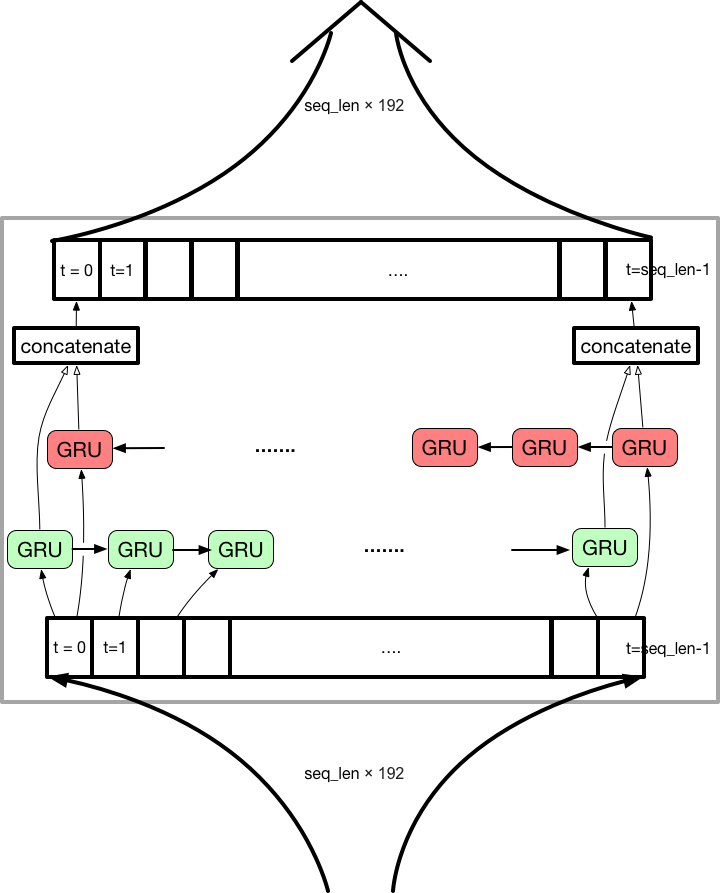
\includegraphics[width=3in]{Figures/rnn_layer}
	\caption[Detail inside recurrent unit]{Illustration of recurrent network}
	\label{fig:rnn_layer}
\end{figure}


\section{Loss and optimizer}
The loss function are composed of three parts, the average cross-entropy loss between predicted secondary structure and true secondary structure, the average cross-entropy loss of solvent accessibility and the summary of all l2 norm  weight regularization. For each protein sequence of length $l$ the loss function formulate as equation \ref{eq:loss}. 
\begin{subequations} 
    \begin{align}
    Loss &=\frac { 1 }{ l } \overset { l }{ \underset { i }{ \Sigma  }  } L_{ s }(s_{ i },s_{ i }^{ * })\quad +\quad \frac { \lambda_1 }{ l } \overset { l }{ \underset { i }{ \Sigma  }  } L_{ a }(a_{ i },a_{ i }^{ * }) \quad +\quad \lambda_2\Sigma\left\| \theta_j \right\|^2 \label{eq:loss}\\
    L_s(s_i, s_i^*) &= -s_i^*log(s_i)\\
    L_a(a_i, a_i^*) &= -a_i^*log(a_i)
    \end{align}	
\end{subequations}
Where $s_i$, $a_i$ represent the predicted secondary structure and solvent accessibility for each residue. $s_i^*$, $a_i^*$ represent is the true label and $\theta_j$ is the weight to be regularized. \par
Adam optimizer \cite{kingma2014adam} are used for training the network.
%\begin{table}[t]
%	\centering
%	\begin{tabular}{|r|l|}
%	\hline
%	7C0 & hexadecimal \\
%	3700 & octal \\ \cline{2-2}
%	11111000000 & binary \\
%	\hline \hline
%	1984 & decimal \\
%	\hline
%	\end{tabular}
%	\caption[Digit representation]{A sample table which will show up in the the List %of Tables as `Digit representation table'; it is set to align at the top of a page}
%\end{table}


%\begin{table}[H]
%	\centering
%	\begin{tabular}{llr}
%	\hline
%	\multicolumn{2}{c}{Item} \\
%	\cline{1-2}
%	Animal & Description & Price (\$) \\
%	\hline
%	Gnat  & per gram & 13.65 \\
%	 & each     &  0.01 \\
%	Gnu   & stuffed  & 92.50 \\
%	Emu   & stuffed  & 33.33 \\
%	Armadillo & frozen & 8.99 \\
%	\hline
%	\end{tabular}
%	\caption[Odd foods]{Another table which will show up in the the List of Tables %as `Odd foods'; it is set to align ``here" in the text.}
%\end{table}



